% ====================================================================
% ФАЙЛ: tasks/03_electrodynamics/capacitors_and_dielectrics_part1.tex
% ТЕМА: ПРОВОДНИКИ И ДИЭЛЕКТРИКИ В ЭЛЕКТРИЧЕСКОМ ПОЛЕ. КОНДЕНСАТОР
% ПАЧКА 1: ВАРИАНТЫ 1–10
% ====================================================================

% === ЗАДАЧА 1 ===
% Тег: #ЭЛЕКТРОДИНАМИКА #КОНДЕНСАТОР #КИМ_11 #ВАРИАНТ_01
\begin{taskbasic}[code={\label{task:elem_cap_v1_n11}}]
\textbf{Задача 1.} Во сколько раз увеличится электроёмкость плоского воздушного конденсатора, если пространство между его пластинами полностью заполнить диэлектриком с диэлектрической проницаемостью $\varepsilon = 4$?

\kim{11}
\end{taskbasic}
\answer{4}

% === ЗАДАЧА 2 ===
% Тег: #ЭЛЕКТРОДИНАМИКА #КОНДЕНСАТОР #КИМ_11 #ВАРИАНТ_02
\begin{taskbasic}[code={\label{task:elem_cap_v2_n11}}]
\textbf{Задача 2.} Какая энергия запасена в конденсаторе электроёмкостью $C = 4\text{ мкФ}$, если напряжение между его обкладками равно $U = 3\text{ В}$? Ответ выразите в микроджоулях (мкДж).

\kim{11}
\end{taskbasic}
\answer{18}

% === ЗАДАЧА 3 ===
% Тег: #ЭЛЕКТРОДИНАМИКА #ПРОВОДНИКИ #КИМ_14 #ВАРИАНТ_07
\begin{taskbasic}[code={\label{task:elem_cap_v7_n14}}]
\textbf{Задача 3.} Незаряженное металлическое тело незамкнутой формы внесли во внешнее однородное электростатическое поле с напряжённостью $\vec{E}_0$. На рисунке показано сечение тела и точки $A, B, C, D$. Из приведённого ниже списка выберите все верные утверждения относительно электростатического состояния тела.

\nopagebreak\smallskip
\begin{center}
\begin{tikzpicture}[scale=1.0, every node/.style={font=\footnotesize}]
    \draw[xstep=1, ystep=1, gray!30, thin] (0,0) grid (5,3);
    
    % Силовые линии внешнего поля
    \draw[-{Stealth[scale=0.8]}, brandPrimary, thick] (0.2,0.6) -- (1.2,0.6);
    \draw[-{Stealth[scale=0.8]}, brandPrimary, thick] (0.2,1.5) -- (1.2,1.5) node[above left] {$\vec{E}_0$};
    \draw[-{Stealth[scale=0.8]}, brandPrimary, thick] (0.2,2.4) -- (1.2,2.4);
    
    % Проводник
    \draw[ultra thick, black, fill=gray!20] (2,0.5) -- (4,0.5) arc (-90:90:1) -- (2,2.5) arc (90:270:0.5) -- cycle;
    
    % Точки
    \fill[black] (1.6,1.5) circle (1.5pt) node[left] {$A$};
    \fill[black] (3,1.5) circle (1.5pt) node[above] {$B$};
    \fill[black] (4.4,1.5) circle (1.5pt) node[right] {$C$};
    \fill[black] (3,0.5) circle (1.5pt) node[below] {$D$};
    
    \node[below left] at (0,0) {0};
\end{tikzpicture}
\end{center}

1) Напряжённость суммарного электрического поля в точке $B$ равна нулю.\\
2) Потенциал электрического поля в точке $A$ больше, чем в точке $C$.\\
3) Концентрация свободных электронов в точке $A$ меньше, чем в точке $C$.\\
4) Напряжённость поля в точке $C$ больше, чем напряжённость внешнего поля $E_0$.\\
5) Потенциалы электрического поля во всех внутренних точках металлического тела одинаковы.

\kim{14}
\end{taskbasic}
\answer{15}

% === ЗАДАЧА 4 ===
% Тег: #ЭЛЕКТРОДИНАМИКА #ПРОВОДНИКИ #КИМ_14 #ВАРИАНТ_08
\begin{taskbasic}[code={\label{task:elem_cap_v8_n14}}]
\textbf{Задача 4.} Незаряженный сплошной металлический цилиндр внесли в однородное электростатическое поле с напряжённостью $\vec{E}_0$, направленной вдоль оси цилиндра. Из приведённого ниже списка выберите все верные утверждения относительно установившегося электростатического состояния системы.

\nopagebreak\smallskip
\begin{center}
\begin{tikzpicture}[scale=1.0, every node/.style={font=\footnotesize}]
    \draw[xstep=1, ystep=1, gray!30, thin] (0,0) grid (5,3);
    
    % Силовые линии внешнего поля
    \draw[-{Stealth[scale=0.8]}, brandPrimary, thick] (0.2,0.8) -- (1.2,0.8);
    \draw[-{Stealth[scale=0.8]}, brandPrimary, thick] (0.2,1.5) -- (1.2,1.5) node[above left] {$\vec{E}_0$};
    \draw[-{Stealth[scale=0.8]}, brandPrimary, thick] (0.2,2.2) -- (1.2,2.2);
    
    % Цилиндр (проекция)
    \draw[ultra thick, black, fill=gray!20] (2,0.8) rectangle (4,2.2);
    
    \node[below left] at (0,0) {0};
\end{tikzpicture}
\end{center}

1) Вектор напряжённости поля внутри цилиндра направлен противоположно вектору $\vec{E}_0$.\\
2) Напряжённость электростатического поля внутри цилиндра равна нулю.\\
3) Правый торец цилиндра зарядится отрицательно.\\
4) Потенциалы электрического поля на левом и правом торцах цилиндра равны.\\
5) Модуль напряжённости электрического поля вблизи торцев цилиндра равен $E_0$.

\kim{14}
\end{taskbasic}
\answer{24}

% ====================================================================
% ФАЙЛ: tasks/03_electrodynamics/capacitors_and_dielectrics_part2.tex
% ТЕМА: ПРОВОДНИКИ И ДИЭЛЕКТРИКИ В ЭЛЕКТРИЧЕСКОМ ПОЛЕ. КОНДЕНСАТОР
% ПАЧКА 2: ВАРИАНТЫ 11–20
% ====================================================================

% === ЗАДАЧА 1 ===
% Тег: #ЭЛЕКТРОДИНАМИКА #КОНДЕНСАТОР #КИМ_11 #ВАРИАНТ_11
\begin{taskbasic}[code={\label{task:elem_cap_v11_n11}}]
\textbf{Задача 1.} Во сколько раз увеличится энергия электрического поля плоского воздушного конденсатора, подключённого к источнику постоянного напряжения, если расстояние между его обкладками уменьшить в $9$ раз?

\kim{11}
\end{taskbasic}
\answer{9}

% === ЗАДАЧА 2 ===
% Тег: #ЭЛЕКТРОДИНАМИКА #КОНДЕНСАТОР #КИМ_11 #ВАРИАНТ_12
\begin{taskbasic}[code={\label{task:elem_cap_v12_n11}}]
\textbf{Задача 2.} Во сколько раз увеличится модуль заряда на обкладках плоского конденсатора, если напряжение между ними увеличить в $2$ раза?

\kim{11}
\end{taskbasic}
\answer{2}

% === ЗАДАЧА 3 ===
% Тег: #ЭЛЕКТРОДИНАМИКА #КОНДЕНСАТОР #КИМ_15 #ВАРИАНТ_15
\begin{taskbasic}[code={\label{task:elem_cap_v15_n15}}]
\textbf{Задача 3.} Плоский воздушный конденсатор ёмкостью $C_0$ подключён к источнику постоянного напряжения $U$. Пространство между пластинами конденсатора полностью заполняют диэлектриком с диэлектрической проницаемостью $\varepsilon = 3$, не отключая конденсатор от источника. Из приведённого ниже списка выберите все верные утверждения относительно произошедших изменений.

\nopagebreak\smallskip
\begin{center}
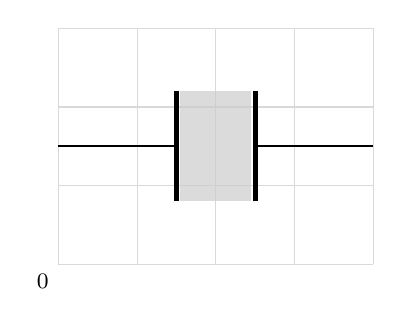
\begin{tikzpicture}[scale=1.0, every node/.style={font=\footnotesize}]
    \draw[xstep=1, ystep=1, gray!30, thin] (0,0) grid (4,3);
    
    % Конденсатор
    \draw[ultra thick, black] (1.5,0.8) -- (1.5,2.2);
    \draw[ultra thick, black] (2.5,0.8) -- (2.5,2.2);
    
    % Подключение к источнику
    \draw[thick, black] (0,1.5) -- (1.5,1.5);
    \draw[thick, black] (2.5,1.5) -- (4,1.5);
    
    % Заполнение диэлектриком
    \fill[gray!40, opacity=0.7] (1.55,0.8) rectangle (2.45,2.2);
    
    \node[below left] at (0,0) {0};
\end{tikzpicture}
\end{center}

1) Электроёмкость конденсатора увеличится в $3$ раза.\\
2) Напряжённость электрического поля между пластинами конденсатора уменьшится в $3$ раза.\\
3) Заряд на пластинах конденсатора увеличится в $3$ раза.\\
4) Энергия электрического поля конденсатора уменьшится в $3$ раза.\\
5) Напряжение между пластинами конденсатора увеличится в $3$ раза.

\kim{15}
\end{taskbasic}
\answer{13}

% === ЗАДАЧА 4 ===
% Тег: #ЭЛЕКТРОДИНАМИКА #КОНДЕНСАТОР #КИМ_25 #ВАРИАНТ_16
\begin{taskbasic}[code={\label{task:elem_cap_v16_n25}}]
\textbf{Задача 4.} Плоский воздушный конденсатор электроёмкостью $C = 2\text{ мкФ}$ заряжен до напряжения $U = 6\text{ В}$ и отключён от источника напряжения. Какую работу необходимо совершить против сил электрического поля, чтобы увеличить расстояние между пластинами конденсатора в $2$ раза? Ответ выразите в микроджоулях (мкДж).

\kim{25}
\end{taskbasic}
\answer{18}

% ====================================================================
% ФАЙЛ: tasks/03_electrodynamics/capacitors_and_dielectrics_part3.tex
% ТЕМА: ПРОВОДНИКИ И ДИЭЛЕКТРИКИ В ЭЛЕКТРИЧЕСКОМ ПОЛЕ. КОНДЕНСАТОР
% ПАЧКА 3: ВАРИАНТЫ 21–30
% ====================================================================

% === ЗАДАЧА 1 ===
% Тег: #ЭЛЕКТРОДИНАМИКА #КОНДЕНСАТОР #КИМ_11 #ВАРИАНТ_21
\begin{taskbasic}[code={\label{task:elem_cap_v21_n11}}]
\textbf{Задача 1.} Во сколько раз уменьшится энергия электрического поля конденсатора постоянной электроёмкости, если напряжение между его обкладками уменьшить в $1{,}5$ раза?

\kim{11}
\end{taskbasic}
\answer{2,25}

% === ЗАДАЧА 2 ===
% Тег: #ЭЛЕКТРОДИНАМИКА #КОНДЕНСАТОР #КИМ_11 #ВАРИАНТ_22
\begin{taskbasic}[code={\label{task:elem_cap_v22_n11}}]
\textbf{Задача 2.} Во сколько раз увеличится модуль заряда на обкладках конденсатора, если его электроёмкость увеличить в $4$ раза, а напряжение между обкладками увеличить в $2$ раза?

\kim{11}
\end{taskbasic}
\answer{8}

% === ЗАДАЧА 3 ===
% Тег: #ЭЛЕКТРОДИНАМИКА #ПРОВОДНИКИ #КИМ_15 #ВАРИАНТ_29
\begin{taskbasic}[code={\label{task:elem_cap_v29_n15}}]
\textbf{Задача 3.} Две металичиские пластины расположенны параллельно друг другу и подключены к полюсам источника постоянного напряжения. Между пластинами помещают незаряженную металлическую пластину меньших размеров. Из приведённого ниже списка выберите все верные утверждения относительно установившегося состояния системы.

\nopagebreak\smallskip
\begin{center}
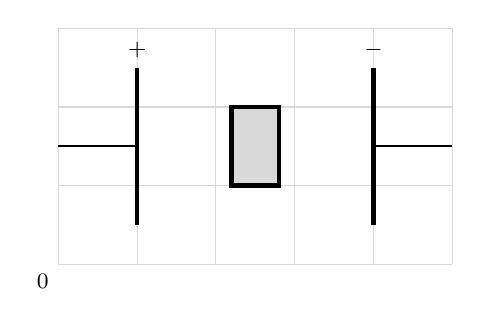
\begin{tikzpicture}[scale=1.0, every node/.style={font=\footnotesize}]
    \draw[xstep=1, ystep=1, gray!30, thin] (0,0) grid (5,3);
    
    % Внешние пластины
    \draw[ultra thick, black] (1,0.5) -- (1,2.5);
    \draw[ultra thick, black] (4,0.5) -- (4,2.5);
    
    % Внутренняя пластина
    \draw[ultra thick, black, fill=gray!30] (2.2,1.0) rectangle (2.8,2.0);
    
    % Подключение внешних пластин
    \draw[thick, black] (0,1.5) -- (1,1.5);
    \draw[thick, black] (4,1.5) -- (5,1.5);
    
    \node[above] at (1,2.5) {$+$};
    \node[above] at (4,2.5) {$-$};
    
    \node[below left] at (0,0) {0};
\end{tikzpicture}
\end{center}

1) Напряжённость электрического поля внутри средней металлической пластины равна нулю.\\
2) Потенциал левой грани средней пластины меньше потенциала её правой грани.\\
3) Модуль напряжённости поля между левой и средней пластинами равен нулю.\\
4) Средняя пластина зарядится положительным суммарным зарядом.\\
5) Потенциалы всех точек внутри средней пластины одинаковы.

\kim{15}
\end{taskbasic}
\answer{15}

% === ЗАДАЧА 4 ===
% Тег: #ЭЛЕКТРОДИНАМИКА #КОНДЕНСАТОР #КИМ_25 #ВАРИАНТ_30
\begin{taskbasic}[code={\label{task:elem_cap_v30_n25}}]
\textbf{Задача 4.} Конденсатор электроёмкостью $C_1 = 4\text{ мкФ}$, заряженный до напряжения $U_1 = 6\text{ В}$, отключают от источника и соединяют параллельно с незаряженным конденсатором электроёмкостью $C_2 = 8\text{ мкФ}$. Какое количество теплоты выделится в соединительных проводах при перераспределении зарядов? Ответ выразите в микроджоулях (мкДж).

\kim{25}
\end{taskbasic}
\answer{36}